\chapter{几何着色器(The Geometry Shader)}
\begin{flushleft}
假设我们没有使用曲面细分阶段,几何着色器阶段是位于顶点和像素着色器阶段之间的可选阶段。顶点着色器输入顶点时,几何着色器输入整个基本体(primitives)。 例如,如果我们绘制三角形列表,那么概念上将为列表中的每个三角形$T$执行几何着色器程序:\\
\end{flushleft}

\begin{lstlisting}
for (UINT i = 0; i < numTriangles; ++i)
  OutputPrimitiveList = GeometryShader(T[i].vertexList);
\end{lstlisting}

\begin{flushleft}
请注意,每个三角形的三个顶点都输入到几何着色器中,几何着色器输出一个基元列表(list of primitives)。 与不能破坏或创建顶点的顶点着色器不同,几何着色器的主要优点是它可以创建或破坏几何体; 这样就可以在GPU上实现一些有趣的效果。 例如,输入基元(primitive)可以扩展为一个或多个其他基元,或者几何着色器可以选择不基于某些条件输出基元。 注意,输出基元不需要与输入基元的类型相同; 例如,几何着色器的常见应用是将点扩展为四边形(两个三角形)。\\

从几何着色器输出的基元由顶点列表定义。 离开几何着色器的顶点位置必须转换为齐次剪辑空间。 在几何着色器阶段之后,我们有一个顶点列表,用于定义齐次剪辑空间中的基元。 投影这些顶点(齐次分割 homogeneous devide),然后像往常一样发生光栅化。
\end{flushleft}

{\large Objectives:}
\begin{itemize}
    \item 1.了解如何编程几何着色器。。
    \item 2.了解如何使用几何着色器有效地实现广告牌。
    \item 3.识别自动生成的基元ID及其某些应用程序。
    \item 4.了解如何创建和使用纹理数组,并了解它们的用途。
    \item 5.要了解alpha-to-coverage如何帮助解决alpha截断的锯齿问题。
\end{itemize}

%-------- 12.1 --------
\section{几何着色器编程(Programming Geometry Shaders)}
\begin{flushleft}
几何着色器编程很像顶点或像素着色器编程,但存在一些差异。以下代码显示了一般形式:\\
\end{flushleft}

\begin{lstlisting}
[maxvertexcount(N)]
void ShaderName (
    PrimitiveType InputVertexType InputName [NumElements],
    inout StreamOutputObject<OutputVertexType> OutputName)
{
    // Geometry shader body...
}
\end{lstlisting}

\begin{flushleft}
我们必须首先指定几何着色器将为单个调用输出的最大顶点数(每个基元调用几何着色器)。 这是通过使用以下属性语法在着色器定义之前设置最大顶点计数来完成的:\\
\end{flushleft}

\begin{lstlisting}
[maxvertexcount(N)]
\end{lstlisting}

\begin{flushleft}
其中$N$是几何着色器为单次调用输出的最大顶点数。几何着色器每次调用可以输出的顶点数是可变的,但不能超过定义的最大值。出于性能考虑,maxvertexcount 应尽可能小; [NVIDIA08]指出GS的峰值性能出现在GS输出1-20标量之间,如果GS输出在27-40个标量之间,性能会下降到50%。每次调用的标量输出数量是maxvertexcount和输出顶点类型结构中标量数量的乘积。在实践中使用这些限制很困难,因此我们可以接受低于峰值的性能,或者选择不使用几何着色器的替代实现;但是,我们还必须考虑替代实现可能具有其他缺点,这仍然可以使几何着色器实现成为更好的选择。此外,[NVIDIA08]中的建议来自2008年(第一代几何着色器),因此现在应该有所改进。\\

几何着色器采用两个参数:输入参数和输出参数。 (实际上,它可能需要更多,这是单独讨论的主题,参见§12.2.4。)输入参数始终是一个顶点数组,它定义一个基元——一个顶点,一个线为两个顶点,三个为a 三角形,四个用于邻接的线,六个用于相邻的三角形。 输入顶点的顶点类型是顶点着色器返回的顶点类型(例如,VertexOut)。 输入参数必须以基本类型为前缀,描述输入到几何着色器中的基元类型。 这可以是以下任何一种:\\
\end{flushleft}

\begin{itemize}
  \item 1.point: 输入基元是点。
  \item 2.line: 输入基元是线段(列表或条带)。
  \item 3.triangle: 输入基元是三角形(列表或条带)。
  \item 4.lineadj: 输入基元是邻接线段(列表或条带)。
  \item 5.triangleadj: 输入基元是邻接三角(列表或条带)。
\end{itemize}

\begin{flushleft}
~\\
NOTICE: 几何着色器中的输入基元始终是完整基元(例如,线的两个顶点和三角形的三个顶点)。 因此,几何着色器不需要区分列表和条带。 例如,如果要绘制三角形条带,则仍会对条带中的每个三角形执行几何着色器,并且每个三角形的三个顶点将作为输入传递到几何着色器中。 这需要额外的开销,因为多个基元共享的顶点在几何着色器中被多次处理。
~\\
输出参数始终具有inout修饰符。 此外,输出参数始终是流类型(stream type)。 流类型存储顶点列表,这些顶点定义几何着色器输出的几何。 几何着色器使用内在的Append方法将一个顶点添加到传出流列表:\\
\end{flushleft}

\begin{lstlisting}
void StreamOutputObject<OutputVertexType>::Append(OutputVertexType v);
\end{lstlisting}

\begin{flushleft}
流类型是模板类型,其中template参数用于指定传出顶点的顶点类型(例如,GeoOut)。 有三种可能的流类型:\\
\end{flushleft}

\begin{itemize}
  \item 1.PointStream<OutputVertexType>: 一个顶点列表定义的点列表(point list)
  \item 2.LineStream<OutputVertexType>: 一个顶点列表定义的线段条带(line strip)
  \item 3.TriangleStream<OutputVertexType>: 一个顶点列表定义的三角条带(triangle strip)
\end{itemize}

\begin{flushleft}
由几何着色器输出的顶点形成基元; 输出基元的类型由流类型(PointStream,LineStream,TriangleStream)指定。 对于线和三角形,输出基元始终是条带。 但是,可以使用内部RestartStrip方法模拟线和三角形列表:\\
\end{flushleft}

\begin{lstlisting}
void StreamOutputObject<OutputVertexType>::RestartStrip();
\end{lstlisting}

\begin{flushleft}
例:如果你想输出三角列表,那么你每次将三个顶点追加到输出流之后都需要调用 RestartStrip 方法。\\

下面是几何着色器签名的例子:\\
\end{flushleft}

\begin{lstlisting}
// EXAMPLE 1: GS ouputs at most 4 vertices. The input
// primitive is a line.
// The output is a triangle strip.
//
[maxvertexcount(4)]
void GS(line VertexOut gin[2],
    inout TriangleStream<GeoOut> triStream)
{
    // Geometry shader body…
}
//
// EXAMPLE 2: GS outputs at most 32 vertices. The
// input primitive is a triangle. The output 
// is a triangle strip.
//
[maxvertexcount(32)]
void GS(triangle VertexOut gin[3],
    inout TriangleStream<GeoOut> triStream)
{
    // Geometry shader body…
}
//
// EXAMPLE 3: GS outputs at most 4 vertices. The input
// primitive is a point. The output is a triangle strip.
//
[maxvertexcount(4)]
void GS(point VertexOut gin[1],
    inout TriangleStream<GeoOut> triStream)
{
    // Geometry shader body…
}
\end{lstlisting}

\begin{figure}[h]
    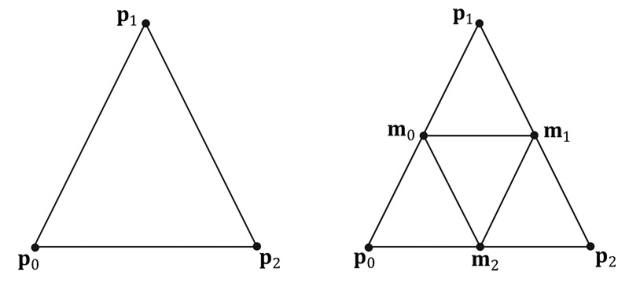
\includegraphics[width=\textwidth]{12-1}
    \centering
    \caption{将三角形细分为四个大小相等的三角形。 观察到三个新顶点是沿着原始三角形边缘的中点。}
    \label{fig:12-1}
\end{figure}

\begin{flushleft}
以下几何着色器说明了Append和RestartStrip方法; 它输入一个三角形,将其细分(图\ref{fig:12-1})并输出四个细分的三角形:\\
\end{flushleft}

\begin{lstlisting}
struct VertexOut
{
    float3 PosL : POSITION;
    float3 NormalL : NORMAL;
    float2 Tex : TEXCOORD;
};
struct GeoOut
{
    float4 PosH : SV_POSITION;
    float3 PosW : POSITION;
    float3 NormalW : NORMAL;
    float2 Tex : TEXCOORD;
    float FogLerp : FOG;
};
void Subdivide(
    VertexOut inVerts[3], 
    out VertexOut
    outVerts[6])
{
    //       1
    //       *
    //     /   \
    //    /     \
    //   m0*–—--*m1
    //  /   \   / \
    // /     \ /   \
    // *–—*–—*
    // 0     m2     2
    VertexOut m[3];
    // Compute edge midpoints.
    m[0].PosL = 0.5f*(inVerts[0].PosL+inVerts[1].PosL);
    m[1].PosL = 0.5f*(inVerts[1].PosL+inVerts[2].PosL);
    m[2].PosL = 0.5f*(inVerts[2].PosL+inVerts[0].PosL);
    // Project onto unit sphere
    m[0].PosL = normalize(m[0].PosL);
    m[1].PosL = normalize(m[1].PosL);
    m[2].PosL = normalize(m[2].PosL);
    // Derive normals.
    m[0].NormalL = m[0].PosL;
    m[1].NormalL = m[1].PosL;
    m[2].NormalL = m[2].PosL;
     // Interpolate texture coordinates.
    m[0].Tex = 0.5f*(inVerts[0].Tex+inVerts[1].Tex);
    m[1].Tex = 0.5f*(inVerts[1].Tex+inVerts[2].Tex);
    m[2].Tex = 0.5f*(inVerts[2].Tex+inVerts[0].Tex);
    outVerts[0] = inVerts[0];
    outVerts[1] = m[0];
    outVerts[2] = m[2];
    outVerts[3] = m[1];
    outVerts[4] = inVerts[2];
    outVerts[5] = inVerts[1];
};
void OutputSubdivision(VertexOut v[6],
    inout TriangleStream<GeoOut> triStream)
{
    GeoOut gout[6];
    [unroll]
    for(int i = 0; i < 6; ++i)
    {
        // Transform to world space space.
        gout[i].PosW = mul(float4(v[i].PosL, 1.0f),
        gWorld).xyz;
        gout[i].NormalW = mul(v[i].NormalL, (float3x3)gWorldInvTranspose);
        // Transform to homogeneous clip space.
        gout[i].PosH = mul(float4(v[i].PosL, 1.0f),
        gWorldViewProj);
        gout[i].Tex = v[i].Tex;
    }
    //       1
    //       *
    //     /   \
    //    /     \
    //   m0*–—--*m1
    //  /   \   / \
    // /     \ /   \
    // *–—*–—*
    // 0     m2     2
    // We can draw the subdivision in two strips:
    // Strip 1: bottom three triangles
    // Strip 2: top triangle
    [unroll]
    for(int j = 0; j < 5; ++j)
    {
        triStream.Append(gout[j]);
    }
    triStream.RestartStrip();
    triStream.Append(gout[1]);
    triStream.Append(gout[5]);
    triStream.Append(gout[3]);
}
[maxvertexcount(8)]
void GS(triangle VertexOut gin[3], inout
    TriangleStream<GeoOut>)
{
    VertexOut v[6];
    Subdivide(gin, v);
    OutputSubdivision(v, triStream);
}
\end{lstlisting}

\begin{flushleft}
几何着色器的编译方式与顶点和像素着色器非常相似。 假设我们在TreeSprite.hlsl中有一个名为GS的几何着色器,那么我们将着色器编译为字节码,如下所示:\\
\end{flushleft}

\begin{lstlisting}
mShaders["treeSpriteGS"] = d3dUtil::CompileShader(
    L"Shaders\\TreeSprite.hlsl", nullptr, "GS", "gs_5_0");
\end{lstlisting}

\begin{flushleft}
与顶点和像素着色器一样,给定的几何着色器作为管道状态对象(PSO)的一部分绑定到渲染管道:\\
\end{flushleft}

\begin{lstlisting}
D3D12_GRAPHICS_PIPELINE_STATE_DESC treeSpritePsoDesc =
    opaquePsoDesc;
...
treeSpritePsoDesc.GS =
{
    reinterpret_cast<BYTE*>(mShaders["treeSpriteGS"]->
        GetBufferPointer()),
    mShaders["treeSpriteGS"]->GetBufferSize()
};
\end{lstlisting}

\begin{flushleft}
~\\
NOTICE: 给定输入基元,几何着色器可以选择不根据某些条件输出它。 通过这种方式,几何体被几何着色器"破坏",这对某些算法很有用。\\
~\\

NOTICE: 如果没有输出足够的顶点来完成几何着色器中的基元,则会丢弃部分基元。\\
\end{flushleft}

%-------- 12.2 --------
\section{树广告牌演示(Tree Billboards demo)}
%-------- 12.2.1 --------
\subsection{概览}





